%%%%%%%%%%%%%%%%%%%%%%%%%%%%%%%%%%%%%%%%%%%%%%%%%%%%%%%%%%%%%%%%%%%%%%%%%
\section{Network Choice Model}  %%%%%%%%%%%%%%%%%%%%%%%%%%%%%%%%%%%%%%%%%
\label{cr:sec:model}

Let $G = (V,E)$ be a directed graph on $n$ nodes (corresponding to items) and $m$ edges.
We denote the out-neighborhood of node $i$ by $N^+_i$ and its in-neighborhood by $N^-_i$.
We consider the following choice process on $G$.
A user starts at a node $i$ and is faced with alternatives $N^+_i$.
The user chooses item $j$ and moves to the corresponding node.
At node $j$, the user is faced with alternatives $N^+_j$ and chooses $k$, and so on.
At any time, the user can stop.
Figure~\ref{cr:fig:samplenet} gives an example of a graph and the alternatives available at a step of the process.

\begin{figure}[t]
  \centering
  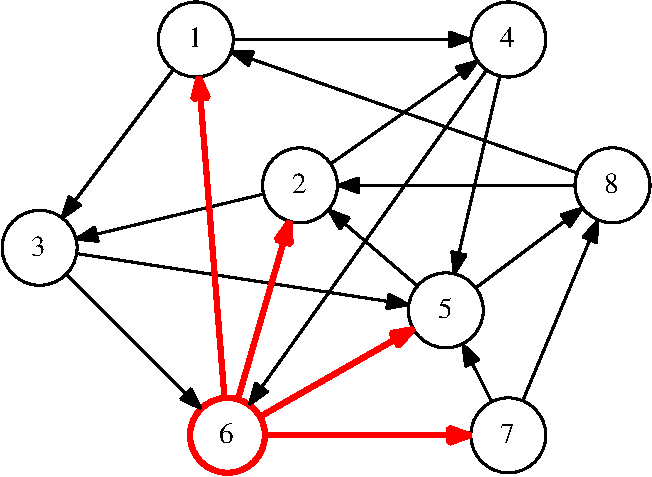
\includegraphics[width=.5\linewidth]{cr-graph-example}
  \caption{An illustration of one step of the process.
  The user is at node 6 and can reach nodes $N^+_6 = \{1, 2, 5, 7\}$.}
  \label{cr:fig:samplenet}
\end{figure}

To define the transition probabilities, we posit Luce's well-known choice axiom that states that the odds of choosing item $j$ over item $j'$ do not depend on the rest of the alternatives \citep{luce1959individual}.
This axiom leads to a unique probabilistic model of choice.
For every node $i$ and every $j \in N^+_i$, the probability that $j$ is selected among alternatives $N^+_i$ can be written as
\begin{align}
\label{cr:eq:singlelik}
p_{ij} = \frac{\lambda_j}{\sum_{k \in N^+_i} \lambda_k}
\end{align}
for some parameter vector $\bm{\lambda} = \begin{bmatrix}\lambda_1 & \cdots & \lambda_n \end{bmatrix}^\transp \in \mathbf{R}_{>0}^n$.
Intuitively, the parameter $\lambda_i$ can be interpreted as the strength (or utility) of item $i$.
Note that $p_{ij}$ depends only on the out-neighborhood of node $i$.
As such, the choice process satisfies the Markov property, and we can think of the sequence of choices as a trajectory in a Markov chain.
In the context of this model, we can formulate the inference problem as follows.
Given a directed graph $G = (V, E)$ and data on the aggregate traffic at each node, find a parameter vector $\bm{\lambda}$ that fits the data.
